\documentclass[en]{article}
\usepackage[left=2.2cm,right=2.2cm,top=2.5cm,bottom=2.5cm]{geometry}
\usepackage[utf8]{inputenc}
\usepackage{minted}
\usepackage{booktabs}
\usepackage{commath}
\usepackage{float}
\usepackage{mathtools}
\usepackage{color}
\usepackage{amsthm}
\usepackage{parskip}


\usepackage[binary-units=true]{siunitx}

\newcommand{\py}[1]{\mintinline{python}{#1}}

\title{Artificial Intelligence (\texttt{LINGI2261}) \\ Assignment 2 --- Group 13}
\author{Martin Braquet, Gilles Peiffer}

\begin{document}

\maketitle

\section{Alpha-Beta search}

\subsection{MiniMax algorithm}

\textcolor{red}{Verification + add details...}

\begin{figure}[H]
 \centering
 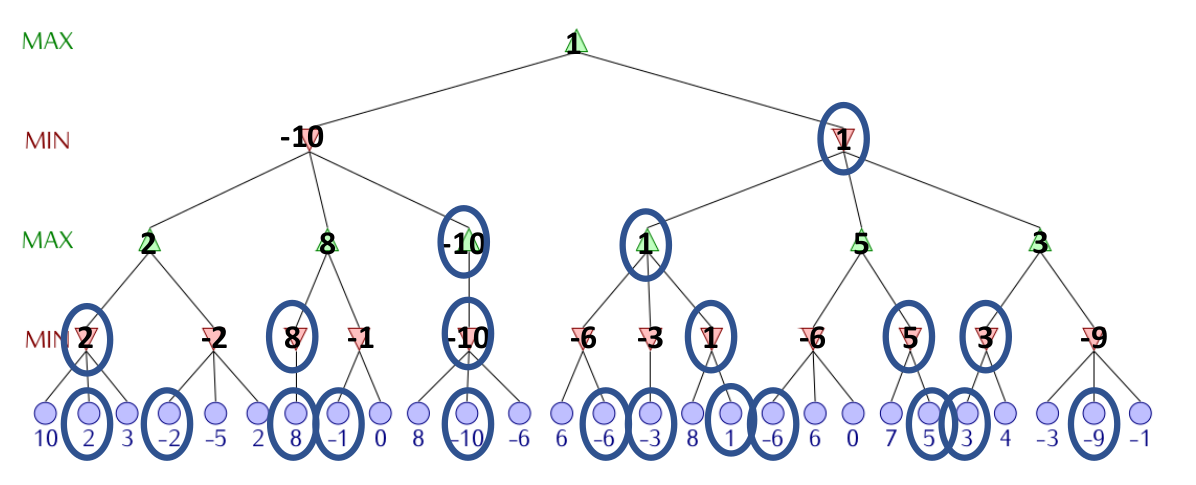
\includegraphics[width=\textwidth]{MiniMax.png}
 \caption{Minimax algorithm}
 \label{fig:minimax}
\end{figure}


\subsection{Alpha-Beta algorithm (left to right)}

\textcolor{red}{Verification + add details...}

\begin{figure}[H]
 \centering
 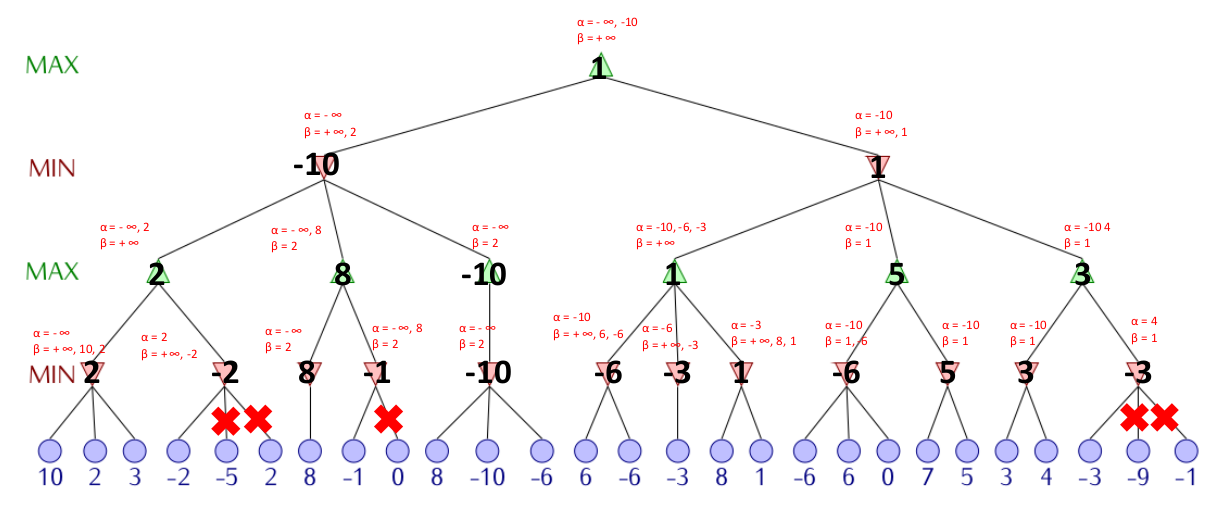
\includegraphics[width=\textwidth]{Alphabeta.png}
 \caption{Alpha-Beta algorithm (left to right)}
 \label{fig:alphabeta}
\end{figure}


\subsection{Alpha-Beta algorithm (right to left)}

\textcolor{red}{Verification + add details...}

\begin{figure}[H]
 \centering
 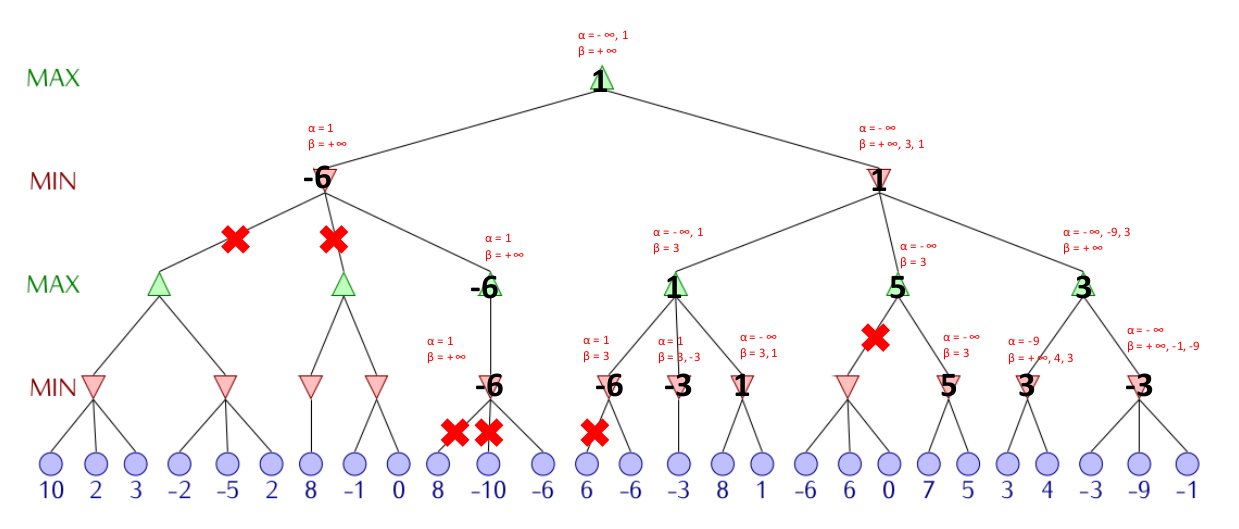
\includegraphics[width=\textwidth]{Alphabeta_reverse.png}
 \caption{Alpha-Beta algorithm (right to left)}
 \label{fig:alphabeta_reverse}
\end{figure}


\subsection{Alpha-Beta algorithm (ordered)}

\textcolor{red}{Verification + add details...}

\begin{figure}[H]
 \centering
 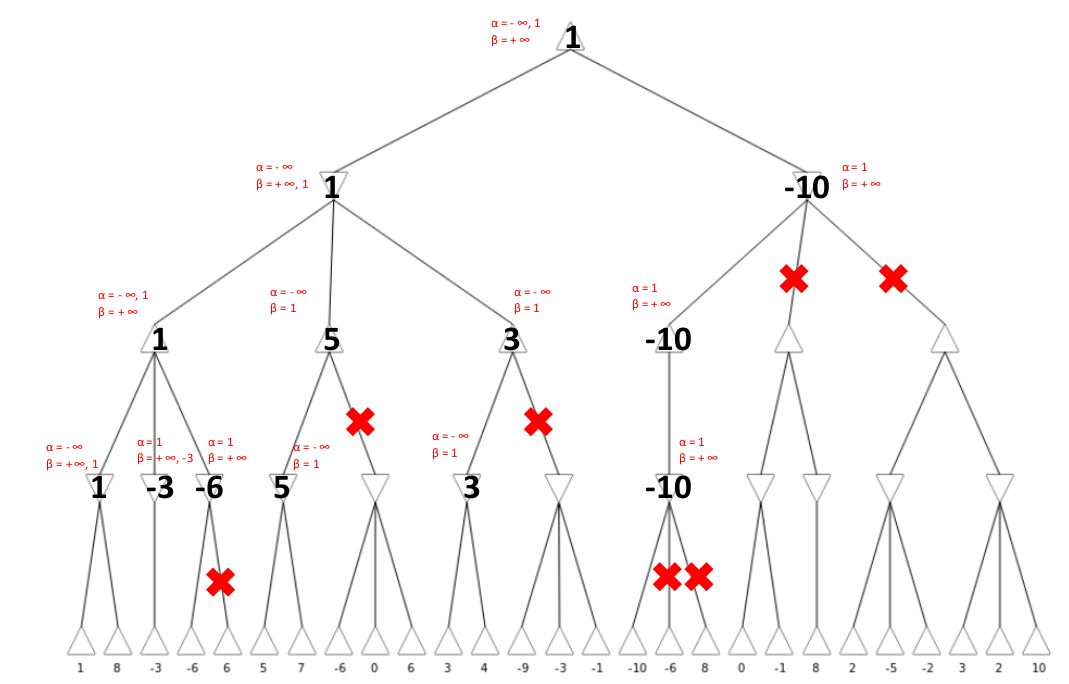
\includegraphics[width=\textwidth]{Alphabeta_ordered.png}
 \caption{Alpha-Beta algorithm}
 \label{fig:alphabeta_ordered}
\end{figure}

\subsection{Alpha-Beta for more than two players}

For more than two players, each node is associated with a tuple giving the value of each player for that state.

Tree pruning is possible if there is an upper bound on the sum of all components of this tuple, and there is a lower bound on the values of each component. We define the sum $S$ as the global upper bound on the sum of all components of the N-tuple, and all components are
assumed to be non-negative. 

The condition \py{v <= alpha} and \py{v >= beta} is now given by \py{Best[Player] >= Bound} where the bound equals the sum $S$ minus the last best node of the upper layer. Indeed, let's take a player 1 from the upper layer which is ensured to get a value of at least $x$ for his layer: $(\ge x, \dots, \dots)$. Then, if player 2 from the lower layer unveils a child with more than $S - x$ for its own value, it will result of a score $(\le x, \ge S - x, \dots)$. Thus, all the remaining children can be dropped since player 1 knows that these children will be chosen by player 2 only if the value of player 1 is less than $x$ \cite{multiplayer}.

\begin{figure}[H]
 \centering
 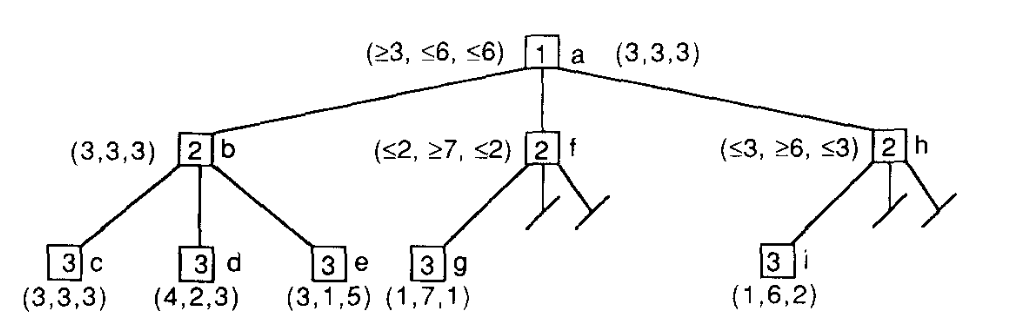
\includegraphics[width=0.7\textwidth]{multiplayer.png}
 \caption{Shallow pruning in three-player game tree \cite{multiplayer}}
 \label{fig:multiplayer}
\end{figure}


\section{Squadro}

\subsection{Comparison of two evaluation functions}

We expect that the new evaluation will work better since it takes into account the opponent, and it will thus prevent the opponent to win for example, by killing his pawns. The old agent is not able to deliberately kill the opponent, consequently decreasing his chances to win.

However, the yellow player still always wins in the four possible starting configurations (which color, who plays first) because he begins with the best paws at the center, progressing by steps of three. The yellow player rapidly puts these paws on the other side, which are then a barrier for the progress of the opponent.
Thus when the depth of the minimax algorithm is not sufficient, the new basic agent is not good enough to overcome the yellow advantage.

\subsection{Cut-off function}

The depth in the \py{minimax.py} implementation is the number of steps along the path from the root node to a node in the layer where we stop the tree search and evaluate the node.

When the depth increases, the new basic agent is able to win even when he is the red player because he can now predict and find a counterattack against the yellow barrier. The new basic agent wins for all starting configurations when the depth is higher than 6.

Since the Squadro contest allows a limited time, we need to select the time allowed for each play.
There exist different methods to choose the maximum time allowed for each search, but an interesting one is to decrease the allowed time troughout the game in order not be out of time in the end. Indeed, we split the time for each play $t_{p}$ following this formula:
\[
    t_{p} = 
    \left\{
    \begin{array}{ll}
      0.2 \: t_{l}^2 & \mathrm{if}\quad t_{l}\leq \SI{100}{s} \\
      20 & \mathrm{otherwise} \\
    \end{array} 
    \right.
\]
where $t_l$ is the remaining time allowed for the considered player. Thus, the time allowed goes well to zero as the remaining time drops.

Using iterative deepening is a good choice to stop the algorithm during its search, it consists to first search 1 ply deep and record the best path of moves. Then it searches 1 ply deeper by increasing the max depth in the manimax algorithm, and could use the recorded path to inform move ordering. In fact, this method only adds a constant fraction to the total search time, which can be compensated by the better move ordering.

The depth is chosen so that the algorithm gives good results, for instance 8. But when time runs out, the program returns the move selected by the deepest completed search.

The cut-off function, which reflects the moment when we need to stop the search, is activated when one of these three conditions is true:

\begin{enumerate}
 \item \py{depth > self.current_depth}: the depth of the analyzed node is higher than the maximum depth,
 \item \py{state.game_over_check()}: the game is over,
 \item \py{time() - self.start_time > self.max_time}: the time elapsed during this search has exceeded the maximum allowed period for this search.
\end{enumerate}

\subsection{Evaluation function}

In the figure presented in the instructions, the yellow basic agent will play the pawn number 3 since it will lead to its highest evaluation: the sum of each pawn’s advancements. However, it is clear that it is not his best move since moving the pawn number 4 would give him the victory. A stronger heuristics has thus to take into account that a player wins if only four of his pawns come back home. In practice, we reduce this progress evaluation to only the four more advanced pawns, bringing a more cogent representation of the state.

\textcolor{red}{Are there any other weak points of the evaluation functions of your basic agents?}

In addition to the sum of each pawn’s advancements, the following features are detailed below.

\begin{itemize}
 \item \textcolor{red}{To complete}
 \item 
 \item 
\end{itemize}



\subsection{Contest}

\bibliographystyle{unsrt}
\bibliography{bib.bib}

\end{document}
